% !TEX root = rob1.tex
\chapter{Regelung von Robotersystemen}
\textbf{Laufende Beobachtung bei der mit den gewonnenen Informationen die Stellgröße derart
verändersot wird, dass trotz Störgrößeneinwirkung die Ausgangsgröße an den gewünschten Verlauf
(Sollverlauf) angeglichen wird.}

\section{Regelkreis}
\begin{figure}[!h]
    \centering
    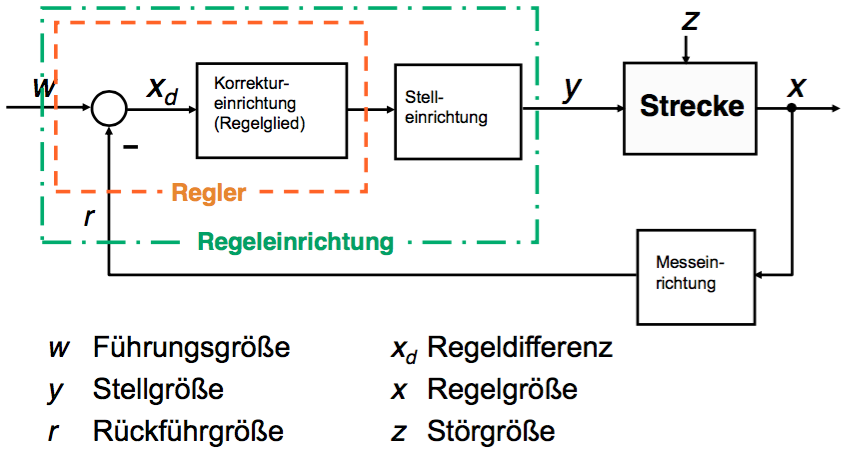
\includegraphics [scale=0.5]{regelkreis}
    \caption{Struktur eines Regelkreises}
\end{figure}

\mparagraph{Wirkungsweise}
\textbf{z} wird größer $\Rightarrow$ \textbf{x} wird gesenkt $\Rightarrow$ \textbf{r} wird abgesenkt
$\Rightarrow$ \textbf{$x_d$} wird angehoben $\Rightarrow$ \textbf{y} wird angehoben $\Rightarrow$
\textbf{x} wird angehoben mit der Tendenz den Sollwert \textbf{$x_s$} wieder anzunehmen. \\
Die Störgröße wird ausgeregelt.

\section{Grundlagen}
\subsection{Laplace Transformation}
\begin{compactitem}
    \item Rechenvereinfachung: Differential und Integralausdrücke werden zu algebraischen Ausdrücken.
    \item Gleichungslösung im Frequenzbereich statt Zeitbereich
    \item Integral muss konvergieren $\rightarrow$ lineare $f(t)$
\end{compactitem}
\begin{displaymath}
     L[f(t)] = f(s) = \int_0^\infty f(t)e^{-st}dt, s := \sigma + j\omega \text{ in } C \text{  } f(t)
      = 0, t < 0
\end{displaymath}

\begin{compactitem}
    \item \textbf{Linearitätssatz}: $L[\alpha f_i(t) + \beta f_2(t)] = \alpha f_1(s) + \beta f_2(s)$
    \item \textbf{Faltungssatz}: $L[f_1(t) * f_2(t)] = f_1(s) * f_2(s)$
    \item \textbf{Grenzwertsatz}: $f_1(t = 0) = \lim_{s \rightarrow \infty} s * f(s)$
    \item \textbf{Differentiationssatz}: $L[\frac{d}{dt}f(t)] = sF(s)$
    \item \textbf{Integrationssatz}: $L[\int f(t)dt] = \frac{1}{s}F(s)$

\end{compactitem}
\subsection{Übertragungsglieder}
\begin{compactitem}
    \item \textbf{P-Glied}: $y(t) = K * u(t)$
    \item \textbf{I-Glied}: $y(t) = K * \int_0^t u(\tau)d\tau$
    \item \textbf{D-Glied}: $y(t) = K * \dot{u}(t)$
    \item \textbf{T$_t$-Glied}: $y(t) = K * u(t-T_t)$
    \item \textbf{S-Glied}: $y(t) = K * \pm u_1(t) \pm u_2(t)$
    \item \textbf{KL-Glied}: $y(t) = K * F(u(t))$
    \item \textbf{M-Glied}: $y(t) = K * u_1(t)u_2(t)$
\end{compactitem}

\section{Reglertypen}
